\section{Exploring Interleaving Space}
\label{s:design}


\newcommand{\segment}{segment graph\xspace}
\newcommand{\segments}{segment graphs\xspace}
\newcommand{\Segments}{Segment graphs\xspace}

\cut{
\begin{itemize}
\item our approach in one sentence: defining the universal set $U$
  using a coverage metric, and directing execution to consume the
  universal set
\item coverage
  \begin{itemize}
  \item rationale:
  \item challenges:
  \item solution:
  \end{itemize}
\item interleaving mutation
  \begin{itemize}
  \item rationale:
  \item challenges:
  \item solution:
  \end{itemize}
\item what do we do to explore the interleaving space?
  \begin{itemize}
  \item We take an interleaving (= a totally ordered instruction sequence as an input)
  \item mutate an interleaving to generate another interleaving
  \item how?
    \begin{itemize}
    \item collect {C1, C2, ...} from the interleaving
    \item infer $U$, the universal set of coverage
    \item consume $U$ until it is empty
    \end{itemize}
  \end{itemize}
\item an intuition for a coverage
  \begin{itemize}
    \item observations
      \begin{itemize}
      \item interleavings are directed acyclic graph
      \item multiple pairs of conflicting accesses are a subgraph of an interleaving
      \end{itemize}
  \item we represent a coverage using a graph (?)
  \end{itemize}

\item an intuition for an interleaving mutation
  \begin{itemize}
  \item two observatrions
    \begin{itemize}
      \item many coverages can be executed together
      \item we can infer what coverages should be further tested
      \end{itemize}
  \item step 1: collect coverage
  \item step 2: inference of coverages to test
  \item step 3: collect coverages that can be tested together
  \item step 4: generate an interleaving to test
  \end{itemize}
\end{itemize}
}


In this section, we describe our approach to explore the interleaving
space.
%
We first provide the overview of our
approach~(\autoref{ss:overview}). Then, we illustrate our coverage
metric in the concurrency dimension~(\autoref{ss:coverage}), and the
instruction scheduling algorithm to quickly saturate the
coverage~(\autoref{ss:scheduler}).

\subsection{Approach Overview}
\label{ss:overview}

\begin{figure*}[ht]
  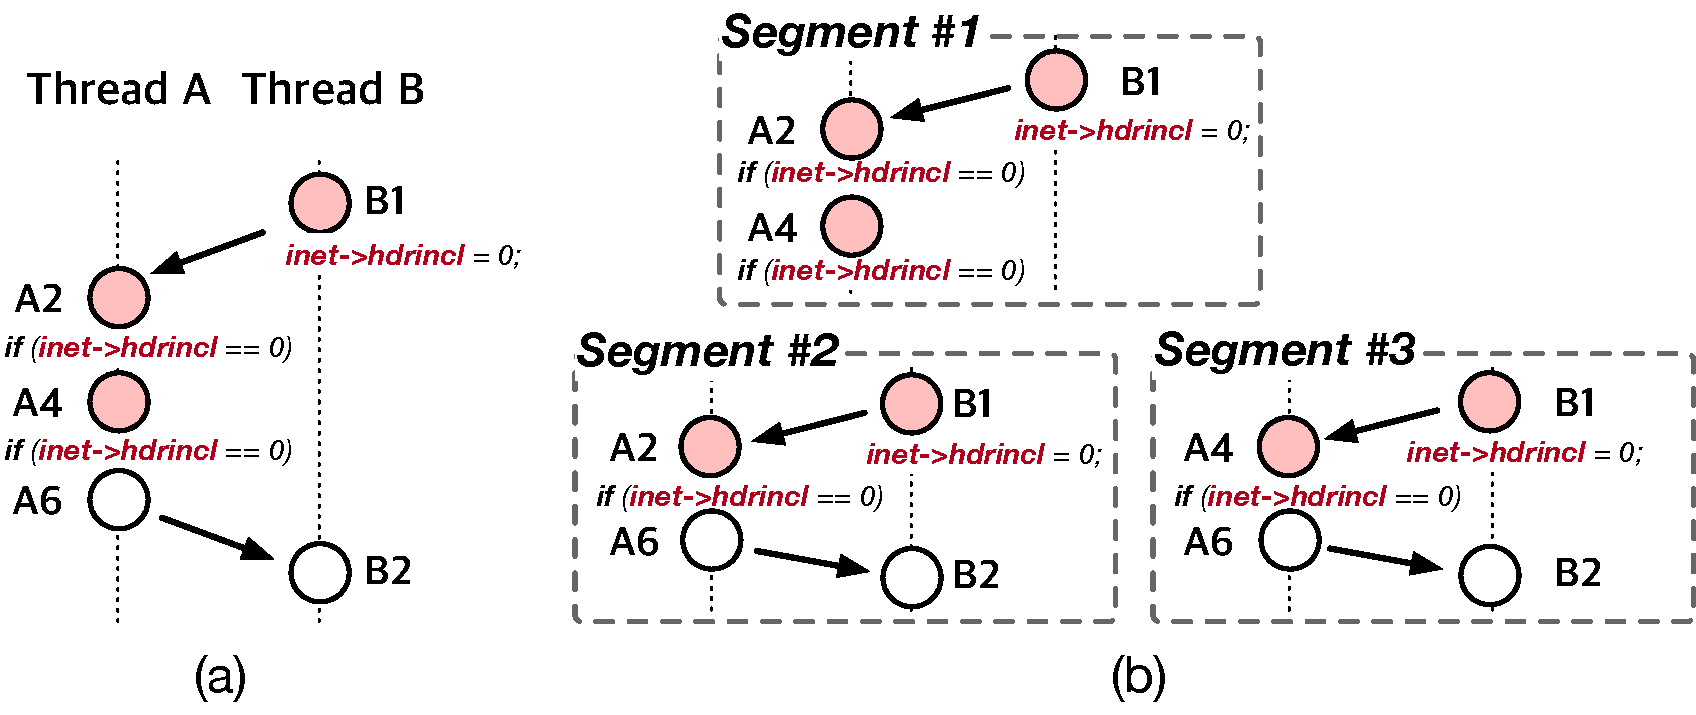
\includegraphics[width=0.9\linewidth]{fig/intuition.pdf}
  \caption{Approach overview to explore the interleaving
    space. \dr{TODO: describe who conflicts with who}}
  \label{fig:overview}
\end{figure*}



Our approach assumes that concurrent jobs (\eg, syscalls) and an
initial interleaving (\eg, a seed interleaving) of the concurrent jobs
are given as an input.
%
With the given input, we deal with the interleaving as a subject of
mutation. In other words, from the given interleaving, we first track
coverage in the concurrency dimension (shortly, concurrency coverage)
that tracks multiple pairs of conflicting accesses. After that, we
generate other interleavings by rescheduling instructions for finding
new concurrency coverage.
%
As a result, we generate various interleavings of the given concurrent
jobs that disclose different concurrency coverage.

\PP{Biconflict coverage}
%
According to the survey~\cite{learningfrommistakes} described in
\autoref{s:motivation}, most race conditions manifest if at most four
memory accesses are executed in a specific order.
%

\dr{TODO: why and how we translate four memory accesses to two
  conflicts?}


\PP{Challenge}
%
% \dr{
% \begin{itemize}
% \item rationale: we need to test muliple pairs of conflicting accesse
% \item challenges: the search space is too large
% \item solution: infer the universal set $U$ and direct the interleaving mutation towards undisclosed coverage
% \end{itemize}
% }
%
One could argue that tracking biconflict coverage is intractable since
the size of the search space is too large.
%
If there are $N$ individual pairs of conflicting accesses, the number
of two pairs of conflicting accesses is propotional to $N^2$, which is
possibly too large to test one-by-one.
%


\dr{Solution}





\PP{Overall steps}
%
\dr{interelaving segment of four instructions?}
%
Let us suppose we have concurrent jobs consisting of \texttt{mmap()}
and \texttt{ioctl(TRANSACTION)} in \autoref{fig:cve-2019-6974}, and
\autoref{fig:overview}-(a) represents an initial interleaving of the
concurrent jobs.
%
As described the figure, the initial interleaving is provided with an
execution order of
$\texttt{A1} \rightarrow \texttt{A2} \rightarrow \texttt{B1}
\rightarrow \texttt{B4} \rightarrow \texttt{B5} \rightarrow
\texttt{A3}$.
%
To recap, the race condition manifests if a condition on the execution
order (\ie,
$(\texttt{A1} \rightarrow \texttt{B1}) \wedge (\texttt{B4} \rightarrow
\texttt{A2})$) is satisfied. In the given interleaving, the race
condition does not manifest since \texttt{A2} is executed before
\texttt{B4}.


With the given input, we first track biconflict coverage.  In the
given interleaving of \autoref{fig:overview}-(a), there are three
individual pairs conflicting accesses,
$\texttt{A1} \rightarrow \texttt{B1}$,
$\texttt{A2} \rightarrow \texttt{B4}$, and
$\texttt{B5} \rightarrow \texttt{A3}$.
%
As described in \autoref{fig:overview}-(b), we compute biconflict
coverage consisting of three segments,
$(\texttt{A1} \rightarrow \texttt{B1}) \wedge (\texttt{A2} \wedge
\texttt{B4})$,
$(\texttt{A1} \rightarrow \texttt{B1}) \wedge (\texttt{B5} \wedge
\texttt{A3})$, and
$(\texttt{A2} \rightarrow \texttt{B4}) \wedge (\texttt{B5} \wedge
\texttt{A3})$.
%
Assuming we initially have empty biconflict coverage, the three
segments are recorded as new coverage of the given interleaivng.



After tracking biconflict coverage from the given interleaving, we
determine whether the interleaving is worth further mutation.
%
To this end, we adopt a strategy to \textit{predict coverage that is
  likley found when the interleaving is mutated}.
%
Taking the example of \autoref{fig:overview}-(c), we can derive
\texttt{Segment 1'} from \texttt{Segment 1} by flipping the execution
order of $\texttt{A2} \rightarrow \texttt{B4}$ to
$\texttt{B4} \rightarrow \texttt{A2}$.
%
Since \texttt{Segment 1'} has not been observed yet, if we run an
interleaving that $\texttt{A1} \rightarrow \texttt{B1}$ and
$\texttt{B4} \rightarrow \texttt{A2}$, we can expand biconflict
coverage with \texttt{Segment 1'}.
%
Similarily, \texttt{Segment 2'} and \texttt{Segment 3'} can be derived
from \texttt{Segment 2} and \texttt{Segment 3}.
%
We denote $U^*$ as a set of segment that are likely covered by
mutations of the interleaving. In this example, \texttt{Segment 1'},
\texttt{Segment 2'}, and \texttt{Segment 3'} are a subset of $U^*$.
%%
If $U^*$ is not empty, we mutate the interleaving toward segments in
$U*$.





Lastly, given $U^*$, we mutate the interleaving by rescheduling memory
access operations in the given interleaving.
%
Since we compute  universal coverage set $U$ 

Our mutation is \textit{directed towards undisclosed coverages in $U$}.

%
And then, to produce other interleavings, our interleaving mutation is










% \subsection{Key Idea}
% \label{ss:keyidea}

% \dr{wip.}
% Our intuition comes from an observation that even a non-failing
% interleaving bears hints on which interleavings require further
% testing.
% %
% For example, if two consecutive load operations reading from a memory
% location are followed by a store operation writing to the same
% location, we can easily deduce that there might be a single-variable
% atomicity violation.
% %
% If we run an interleaving generated by rearranging these operations,
% we can identify whether the atomicity violation actually occurs or
% not.
% %
% Our approach to explore the interleaving space realizes this
% intuition.



% \PP{Overall steps}
% %
% Let us assume we obtain a totally ordered instruction sequence after
% executing concurrent jobs~(\autoref{fig:intuition}-(a)).
% %
% In this instruction sequence, our purposes are 1) to track an
% interesting behavior of the sequence, and 2) to schedule instructions
% in the sequence for exposing more interesting behaviors.


% As to tracking interesting behaviors, we follow the survey mentioned
% in \autoref{ss:motivation} describing that most race conditions
% deterministically manifest depending on a specific partial order of at
% most four memory accesses.
% %
% According to this survey, such partial orders are ``interesting''
% behaviors as they have a strong correlation to manifestation of
% concurrency bugs.
% %
% Therefore, our purpose in tracking interesting behaviors in the
% concurrency dimension turns into identifying how such partial orders
% are established in the given sequence.
% %
% To this end, we enumerate small groups of a few (\eg, four) memory
% accesses brought in the given instruction
% sequence~(\autoref{fig:intuition}-(b)).
% %
% As the execution order of memory accesses in each group are already
% determined, each group explains a part of the interleaving, therefore,

% %
% During fuzzing, we keep tracking segments as the signal of new
% interelavings of concurrent jobs.





% After collecting segments of concurrent jobs, we need to run the
% concurrent jobs with different interleaving to observe different
% segments.
% %
% Instead of blindly scheduling instructions, we deduce what partial
% orders need to be explored in advance.
% %
% In other words, we hypothesize imaginary segments derived from
% collected segments for further testing~(\autoref{fig:intuition}-(c)).
% %
% For example, by rearranging instructions of \texttt{Segment 1}, we
% derive an imaginary segment called \texttt{Segment 1'} that are not
% yet observed.
% %
% These imaginary segments will be used as scheduling hints; our
% instruction scheduling mechanism will enforce imaginary segments
% during further fuzzing runs.
% %
% It is worth noting that segments may be identical since the execution
% order of not-conflicting instructions does not affect the outcome.
% %
% In this example, \texttt{Segment 1'} and \texttt{Segment 1''} are
% identical and we consider they are redundant.

% As a last step, we generate a hypothetical interleaving containing
% these imaginary segments and run the interleaving to observe an
% outcome~(\autoref{fig:intuition}-(d)).
% %
% Among all imaginary segments, some of them can be enforced together,
% while some cannot.  For example, \texttt{Segment 1'} and
% \texttt{Segment 2'} may be enforced together as they do not make a
% conflict on the execution order of instructions.
% %
% We call two imaginary segments are harmonious if they are able to be
% enforced together.
% %
% As all imaginary segments are not harmonious to all others, we need to
% run different interleavings multiple times. For each fuzzing run, we
% repeat generating a hypothetical interleaving by gathering harmonious
% segments until we consume all imaginary segments.

% \PP{Interleaving in a graph form}
% %
% Our interleaving exploration mechanism requires a few operations on an
% interleaving such as 1) rearranging instructions in a segment, 2)
% gathering harmonious segments, and 3) generating a whole interleaving
% carrying multiple segments.
% %
% We notice that if we consider an interleaving as a graph of partial
% orders, all above operations become simple graph operations.

% From a given interleaving, we draw a graph consisting of vertices
% representing memory access operations and edges representing the
% execution order of the operations that may change the outcome if
% reversed.
% %
% \dr{explain more intuition:}
% With this graph, the required operations are simplified as follows: 1)
% rearranging instructions is done by changing the direction of edges,
% 2) we can determine segments are harmonious if there is no loop in a
% graph, and 3) a topological sort on a grpah generates a whole
% interleaving.


% In the rest of this section, we define the graph form of an
% interleaving, and then provide details of the interleaving mutation.




\subsection{Biconflict Coverage}
\label{ss:coverage}

\newcommand{\mutable}{mutable edge\xspace}
\newcommand{\mutables}{mutable edges\xspace}
\newcommand{\immutable}{immutable edge\xspace}
\newcommand{\immutables}{immutable edges\xspace}

\begin{itemize}
\item how?
  \begin{itemize}
  \item collect {C1, C2, ...} from the interleaving
  \item infer $U$, the universal set of coverage
  \item consume $U$ until it is empty
  \end{itemize}
\item an intuition for a coverage
  \begin{itemize}
  \item observations
    \begin{itemize}
    \item interleavings are directed acyclic graph
    \item multiple pairs of conflicting accesses are a subgraph of an interleaving
    \end{itemize}
  \item we represent a coverage using a graph (?)
  \end{itemize}
\end{itemize}



\begin{figure}[t]
  \caption{interleaving graph}
  \label{fig:interleaving-graph}
\end{figure}

In order to represent a partial order of memory accesses, we propose a
form of directed acyclic graph (DAG) called interleaving graph.
%
An interleaving graph describes an interleaving of concurrent jobs,
and represents partial orders between instructions.
%
In an interleaving graph, vertices indicate memory access operations,
and edges represent partial orders between these operations.
%
If there is a path from a vertex from another vertex, then the
execution order of two operations is established.

We categorize edges into two types, called \immutables and \mutables.
%
A \immutable corresponds to a program order in which instructions
appear on a thread~\cite{frightening, lkmm}. As a program order is
defined between instructions executed by the same thread, all
\immutables connect instructions from the same thread.
%
On the other hand, a \mutable is responsible to connect conflicting
instructions that 1) are executed by different threads, 2) access the
same memory location, and 3) at least one of them is write.
%
Therefore, the execution order of instructions connected by a \mutable
may directly affect the behavior of a program.


\autoref{fig:interleaving-graph} shows an example of an interleaving
graph.
%
\dr{TODO:}


\dr{TODO: imprecise description}
%
In terms of interleaving, \immutables and \mutables have different
properties. Let us suppose we have two interleaving graphs derived
from different interleavings of the same concurrent jobs.
%
As \immutables represent program orders, direction of \immutables does
not differ in the two interleaving graphs.
%
Whereas, a direction of \mutables may be different in the two
interleaving graphs.
%
It is worth noting that an edge may appear in only one interleaving
graph regardless of its type. This is because the control flow may be
changed according to the change of the data flow.


\PP{Segment of interleaving graph as coverage}
%
Although all execution order of conflicting instructions (\ie,
\mutables) in an interleaving graph may affect an outcome, we
concentrate on a small number of instructions because a few
instructions are enough to cause most ``interesting'' behaviors, \ie,
race conditions.

\dr{divide?}
%
We thus divide the interleaving graph into a set of subgraphs called
interleaving segment graphs, short for \segments.
%
While the interleaving graph represents a whole interleaving, an
\segment is a subgraph of the given interleaving graph that contains
two \mutables and at most four vertices. In addition, vertices in a
\segment are connected by at least one \mutable.

We capture \segments as coverage of a given interleaving of concurrent
jobs.
%
If a new \segment is not found while continuing to run the concurrent
jobs with different interleavings, the concurrent jobs unlikely expose
a race condition. In other words, if we collect all \segments of
concurrent jobs, we can lower the priority of the concurrent jobs.
%
It is worth noting that we select four as the maximum number of
vertices in a \segment because not only it is enough for most race
conditions, but also \dr{}...

In order to identify \segments from execution, we need to know the
total order of memory accesses. Otherwise, we may miss the execution
order between instructions so cannot faithfully capture \segments.
%
Therefore, our scheduling mechanism serializes execution of concurrent
jobs during fuzzing. Details are described later in \autoref{s:impl}.


\subsection{Interleaving Mutation}
\label{ss:scheduler}


% \textit{estimates
%   the universal coverage set $U$}, a set of fragment that the given
% concurrent jobs possibly execute.

% If the universal coverage set $U$ contains coverage that are not yet
% observed, we determine that the interleaving is worthy of further
% mutating.


\begin{itemize}
\item an intuition for an interleaving mutation
  \begin{itemize}
  \item two observatrions
    \begin{itemize}
      \item many coverages can be executed together
      \item we can infer what coverages should be further tested
      \end{itemize}
  \item step 1: collect coverage
  \item step 2: inference of coverages to test
  \item step 3: collect coverages that can be tested together
  \item step 4: generate an interleaving to test
  \end{itemize}
\end{itemize}



% Since concurrent jobs may reveal different behaviors depending on an
% interleaving, a concurrency fuzzer adopt additional mutation strategy
% called interleaving mutation.

Our interleaving mutation is designed in a different way from previous
studies.
%
Instead of randomly selecting scheduling points~\cite{krace, ski} or
changing the execution order of a few instructions~\cite{razzer,
  snowboard}, we draw a whole hypothetical interleaving directed
towards uncaptured \segments.
%
To this end, our interleaving mutation consists of three steps:
%
1) identifying uncaptured \segments, 2) selecting \textit{harmonious}
\segments, and 3) generating scheduling points to test the selected
\segments.

\PP{Identifying uncaptured segment graphs}
%
Given \segments derived from an interleaving, identifying uncaptured
\segments is the first step of interleaving mutation for generating
another interleaving.
%
For each \segment, we change directions of \mutables to infer
uncaptured \segments.
%
As each \segment contains two \mutables, at most four uncaptured
\segments are derived for one \segment.

\dr{TODO:}...






\PP{Selecting interleaving segments to direct}
%
Given all uncaptured \segments, it is unlikely that all \segments can
be tested at once.
%
Our approach is to find out a subset of \segments that are
\textit{harmonious}. \Segments are harmonious if they do not form a
cycle in an imaginary graph.


It may require heavy computation to identify the largest subset that
are all harmonious to each other.
%
Instead of finding the optimal solution, we choose to use a greedy
algorithm.
%
Especially, given uncaptured \segments extracted from an interleaving
graph, our interleaving mutation starts by selecting a random
\segment.
%
And then it iteratively selects a \segment while confirming that the
selected \segment is harmonious.
%
Determining a given \segment is harmonious is conducted by checking a
loop in an accumulated interleaving graph.

\dr{TODO: describe an algorithm to check a loop. }
Its time complexity is $O(V)$.


\PP{Generating scheduling points}
%
After selecting harmonious \segments, generating scheduling points can
be easily done by conducting a topological
sort~\cite{topologicalsort}.
%
Since an imaginary interleaving graph is acyclic, a topological sort
always returns a sequence of vertices (\ie, instructions) that does
not violate a program order.
%
It is well known that the time complexity of a topological sort is
$O(V+E)$. Considering that the graph is sparse, $E$ is a small value
so the time complexity can be asymptotically considered as $O(V)$.
%
In this sequence, scheduling points are just instructions that the
preemption should happen; \ie, the next instruction is executed by a
different thread.
%


\dr{TODO: what if scheduling points are missing}


%%% Local Variables:
%%% mode: latex
%%% TeX-master: "p"
%%% End:
